% Generated on 2025-04-15 18:19:14 by gEcon ver. 1.2.1 (2023-01-18)
% http://gecon.r-forge.r-project.org/

% Model name: NK_RS

\section{Steady-state values}


\begin{tabular}{c|c|}
  & Steady-state value\\
\hline
$\epsilon^{\mathrm{G}}$ & 1 \\
$g^{\mathrm{1}}$ & 7.3514 \\
$g^{\mathrm{2}}$ & 4.9009 \\
${i\!n\!f\!l\!a\!t\!i\!o\!n}^{\mathrm{gap}}$ & 1 \\
$\lambda$ & 1.5467 \\
${m\!c}$ & 0.6667 \\
$\nu^{\mathrm{p}}$ & 1 \\
${p\!e\!r\!c\!i\!e\!v\!e\!d}^{\pi^{\mathrm{obj}}}$ & 1 \\
$\pi$ & 1 \\
$\pi^{\star}$ & 1 \\
$\pi^{\mathrm{obj}}$ & 1 \\
${p\!H}$ & 0.95 \\
${p\!L}$ & 0.05 \\
$q$ & 1.5467 \\
$r$ & 0.0351 \\
$B$ & 0 \\
$C$ & 0.3255 \\
${D\!i\!v}$ & 0.1601 \\
$G$ & 0.0865 \\
$I$ & 0.0684 \\
$K^{\mathrm{s}}$ & 2.7374 \\
$L^{\mathrm{s}}$ & 0.2279 \\
$Q$ & 1 \\
$R$ & 1.0101 \\
$T$ & 0.0865 \\
$U$ & -167.8256 \\
$W$ & 0.9837 \\
$Y$ & 0.4804 \\
$Y^{\mathrm{j}}$ & 0.4804 \\
$Y^{\mathrm{s}}$ & 0.4804 \\
$Z$ & 1 \\
\hline
\end{tabular}


\section{The solution of the 1st order perturbation}

\subsection*{Matrix $P$}

$$\bordermatrix{
~ & \epsilon^{\mathrm{G}}_{t-1} & \nu^{\mathrm{p}}_{t-1} & {p\!e\!r\!c\!i\!e\!v\!e\!d}^{\pi^{\mathrm{obj}}}_{t-1} & \pi_{t-1} & \pi^{\mathrm{obj}}_{t-1} & B_{t-1} & K^{\mathrm{s}}_{t-1} & R_{t-1} & Z_{t-1} \cr
\epsilon^{\mathrm{G}}_{t} & 0.949 & 0 & 0 & 0 & 0 & 0 & 0 & 0 & 0 \cr
\nu^{\mathrm{p}}_{t} & 0 & 0.908 & 0 & 0 & 0 & 0 & 0 & 0 & 0 \cr
{p\!e\!r\!c\!i\!e\!v\!e\!d}^{\pi^{\mathrm{obj}}}_{t} & 0 & 0.0002 & 0.0498 & 0.0014 & 0.0071 & 0 & -0.0002 & -0.0047 & -0.0003 \cr
\pi_{t} & -0.0001 & 0.0549 & 0 & 0.3347 & 1.6743 & 0 & -0.0399 & -1.1151 & -0.0644 \cr
\pi^{\mathrm{obj}}_{t} & 0 & 0 & 0 & 0 & 0.9999 & 0 & 0 & 0 & 0 \cr
B_{t} & 0 & 0 & 0 & 0 & 0 & 0 & 0 & 0 & 0 \cr
K^{\mathrm{s}}_{t} & 0.0052 & 0.5527 & 0.0001 & -1.2493 & 15.5761 & 0 & 0.4384 & -15.1013 & -0.4031 \cr
R_{t} & 0.0006 & 0.0147 & 0 & 0.0313 & 0.4011 & 0 & -0.0135 & 0.5465 & -0.011 \cr
Z_{t} & 0 & 0 & 0 & 0 & 0 & 0 & 0 & 0 & 0.823 \cr
}$$

\subsection*{Matrix $Q$}

$$\bordermatrix{
~ & \epsilon^{\mathrm{Z}} & \eta^{\mathrm{p}} & \eta^{\mathrm{R}} & \eta^{\pi} & \eta^{\mathrm{G}} \cr
\epsilon^{\mathrm{G}} & 0 & 0 & 0 & 0 & 1 \cr
\nu^{\mathrm{p}} & 0 & 0 & 0 & 0 & 0 \cr
{p\!e\!r\!c\!i\!e\!v\!e\!d}^{\pi^{\mathrm{obj}}} & -0.0003 & 0.0001 & -0.0049 & 0.0071 & 0 \cr
\pi & -0.0783 & 0.0121 & -1.1604 & 1.6745 & -0.0001 \cr
\pi^{\mathrm{obj}} & 0 & 0 & 0 & 1 & 0 \cr
B & 0 & 0 & 0 & 0 & 0 \cr
K^{\mathrm{s}} & -0.4898 & -0.0064 & -15.7141 & 15.5777 & 0.0055 \cr
R & -0.0133 & -0.0002 & 0.5687 & 0.4012 & 0.0007 \cr
Z & 1 & 0 & 0 & 0 & 0 \cr
}$$

\subsection*{Matrix $R$}

$$\bordermatrix{
~ & \epsilon^{\mathrm{G}}_{t-1} & \nu^{\mathrm{p}}_{t-1} & {p\!e\!r\!c\!i\!e\!v\!e\!d}^{\pi^{\mathrm{obj}}}_{t-1} & \pi_{t-1} & \pi^{\mathrm{obj}}_{t-1} & B_{t-1} & K^{\mathrm{s}}_{t-1} & R_{t-1} & Z_{t-1} \cr
g^{\mathrm{1}}_{t} & 0.1474 & 0.9164 & 0.0002 & -1.9772 & 30.4198 & 0 & -0.8826 & -15.6826 & -0.8627 \cr
g^{\mathrm{2}}_{t} & 0.1474 & 0.9164 & 0.0002 & -1.9772 & 30.4198 & 0 & -0.8826 & -15.6826 & -0.8627 \cr
{i\!n\!f\!l\!a\!t\!i\!o\!n}^{\mathrm{gap}}_{t} & -0.0001 & 0.0547 & -0.0498 & 0.3333 & 1.6672 & 0 & -0.0398 & -1.1104 & -0.0642 \cr
\lambda_{t} & 0.1179 & 0.1359 & -0.0001 & 0.8044 & -9.5958 & 0 & -0.2745 & 9.2056 & -0.0385 \cr
{m\!c}_{t} & 0.0862 & 4.9708 & 0.0007 & -10.2156 & 126.7452 & 0 & -4.181 & -122.7415 & -4.7403 \cr
\pi^{\star}_{t} & -0.0012 & 0.5419 & 0.0001 & -1.3251 & 16.5247 & 0 & -0.3941 & -11.006 & -0.636 \cr
{p\!H}_{t} & 0.0001 & -0.0273 & 0.0249 & -0.1667 & -0.8336 & 0 & 0.0199 & 0.5552 & 0.0321 \cr
{p\!L}_{t} & -0.0011 & 0.5194 & -0.4729 & 3.1666 & 15.8386 & 0 & -0.3778 & -10.549 & -0.6096 \cr
q_{t} & 0.1179 & 0.1359 & -0.0001 & 0.8044 & -9.5958 & 0 & -0.2745 & 9.2056 & -0.0385 \cr
r_{t} & 0.2504 & 9.6818 & 0.0012 & -19.1237 & 237.5426 & 0 & -8.6795 & -230.101 & -7.5809 \cr
C_{t} & -0.0534 & 0.9652 & 0.0002 & -2.6415 & 32.5391 & 0 & -0.6513 & -31.4584 & -0.8022 \cr
{D\!i\!v}_{t} & -0.0082 & -7.9545 & -0.0007 & 11.5232 & -142.6932 & 0 & 4.8635 & 138.1235 & 6.6399 \cr
G_{t} & 0.949 & 0 & 0 & 0 & 0 & 0 & 0 & 0 & 0 \cr
I_{t} & 0.2078 & 22.1074 & 0.0033 & -49.972 & 623.0451 & 0 & -21.4623 & -604.0518 & -16.1258 \cr
L^{\mathrm{s}}_{t} & 0.2346 & 6.7301 & 0.0008 & -12.7258 & 158.2819 & 0 & -5.4265 & -153.3708 & -5.2337 \cr
Q_{t} & 0 & 0 & 0 & 0 & 0 & 0 & 0 & 0 & 0 \cr
T_{t} & 0.949 & 0 & 0 & 0 & 0 & 11.5637 & 0 & 0 & 0 \cr
U_{t} & -0.0107 & -0.0272 & 0 & -0.0234 & 0.2831 & 0 & 0.0226 & -0.1954 & 0.0162 \cr
W_{t} & 0.0158 & 2.9517 & 0.0004 & -6.3979 & 79.2607 & 0 & -2.2531 & -76.7303 & -2.3471 \cr
Y_{t} & 0.1642 & 3.8031 & 0.0006 & -8.9081 & 110.7973 & 0 & -3.4985 & -107.3595 & -2.8406 \cr
Y^{\mathrm{j}}_{t} & 0.1642 & 4.7111 & 0.0006 & -8.9081 & 110.7973 & 0 & -3.4985 & -107.3595 & -2.8406 \cr
Y^{\mathrm{s}}_{t} & 0.1642 & 4.7111 & 0.0006 & -8.9081 & 110.7973 & 0 & -3.4985 & -107.3595 & -2.8406 \cr
}$$

\subsection*{Matrix $S$}

$$\bordermatrix{
~ & \epsilon^{\mathrm{Z}} & \eta^{\mathrm{p}} & \eta^{\mathrm{R}} & \eta^{\pi} & \eta^{\mathrm{G}} \cr
g^{\mathrm{1}} & -1.0482 & 0.1094 & -16.319 & 30.4228 & 0.1553 \cr
g^{\mathrm{2}} & -1.0482 & -0.0266 & -16.319 & 30.4228 & 0.1553 \cr
{i\!n\!f\!l\!a\!t\!i\!o\!n}^{\mathrm{gap}} & -0.078 & 0.012 & -1.1555 & 1.6674 & -0.0001 \cr
\lambda & -0.0468 & 0.0052 & 9.5791 & -9.5967 & 0.1243 \cr
{m\!c} & -5.7597 & -0.0537 & -127.7227 & 126.7579 & 0.0908 \cr
\pi^{\star} & -0.7728 & 0.1192 & -11.4526 & 16.5264 & -0.0012 \cr
{p\!H} & 0.039 & -0.006 & 0.5777 & -0.8337 & 0.0001 \cr
{p\!L} & -0.7407 & 0.1142 & -10.9771 & 15.8402 & -0.0012 \cr
q & -0.0468 & 0.0052 & 9.5791 & -9.5967 & 0.1243 \cr
r & -9.2113 & -0.0999 & -239.4392 & 237.5663 & 0.2638 \cr
C & -0.9748 & -0.0144 & -32.735 & 32.5424 & -0.0563 \cr
{D\!i\!v} & 8.0679 & 0.0612 & 143.7289 & -142.7074 & -0.0086 \cr
G & 0 & 0 & 0 & 0 & 1 \cr
I & -19.594 & -0.2554 & -628.5659 & 623.1074 & 0.2189 \cr
L^{\mathrm{s}} & -6.3594 & -0.066 & -159.595 & 158.2977 & 0.2472 \cr
Q & 0 & 0 & 0 & 0 & 0 \cr
T & 0 & 0 & 0 & 0 & 1 \cr
U & 0.0197 & -0.0003 & -0.2033 & 0.2831 & -0.0113 \cr
W & -2.8519 & -0.0339 & -79.8442 & 79.2686 & 0.0167 \cr
Y & -3.4515 & -0.0462 & -111.7165 & 110.8084 & 0.173 \cr
Y^{\mathrm{j}} & -3.4515 & -0.0462 & -111.7165 & 110.8084 & 0.173 \cr
Y^{\mathrm{s}} & -3.4515 & -0.0462 & -111.7165 & 110.8084 & 0.173 \cr
}$$


\section{Model statistics}

\subsection{Basic statistics}

\begin{tabular}{c|c|c|c|c|}
  & Steady-state value & Std. dev. & Variance & Loglin\\
\hline
$\epsilon^{\mathrm{G}}$ & 1 & 1.3033 & 1.6986 & Y    \\
$g^{\mathrm{1}}$ & 7.3514 & 33.2682 & 1106.7707 & Y    \\
$g^{\mathrm{2}}$ & 4.9009 & 33.268 & 1106.7604 & Y    \\
${i\!n\!f\!l\!a\!t\!i\!o\!n}^{\mathrm{gap}}$ & 1 & 2.0394 & 4.1593 & Y    \\
$\lambda$ & 1.5467 & 16.9702 & 287.9891 & Y    \\
${m\!c}$ & 0.6667 & 174.7432 & 30535.1868 & Y    \\
$\nu^{\mathrm{p}}$ & 1 & 0 & 0 & Y    \\
${p\!e\!r\!c\!i\!e\!v\!e\!d}^{\pi^{\mathrm{obj}}}$ & 1 & 0.0089 & 0.0001 & Y    \\
$\pi$ & 1 & 2.0483 & 4.1954 & Y    \\
$\pi^{\star}$ & 1 & 18.6165 & 346.574 & Y    \\
$\pi^{\mathrm{obj}}$ & 1 & 1.2917 & 1.6684 & Y    \\
${p\!H}$ & 0.95 & 1.0197 & 1.0398 & Y    \\
${p\!L}$ & 0.05 & 19.3745 & 375.373 & Y    \\
$q$ & 1.5467 & 16.9702 & 287.9891 & Y    \\
$r$ & 0.0351 & 336.2675 & 113075.8376 & Y    \\
$B$ & 0 & 0 & 0 & N    \\
$C$ & 0.3255 & 42.2117 & 1781.8288 & Y    \\
${D\!i\!v}$ & 0.1601 & 198.2823 & 39315.8834 & Y    \\
$G$ & 0.0865 & 1.3033 & 1.6986 & Y    \\
$I$ & 0.0684 & 868.2099 & 753788.4129 & Y    \\
$K^{\mathrm{s}}$ & 2.7374 & 27.5518 & 759.1001 & Y    \\
$L^{\mathrm{s}}$ & 0.2279 & 220.2747 & 48520.9583 & Y    \\
$Q$ & 1 & 0 & 0 & Y    \\
$R$ & 1.0101 & 0.8977 & 0.8059 & Y    \\
$T$ & 0.0865 & 1.3033 & 1.6986 & Y    \\
$U$ & -167.8256 & 0.8178 & 0.6688 & Y    \\
$W$ & 0.9837 & 106.2007 & 11278.5832 & Y    \\
$Y$ & 0.4804 & 151.3211 & 22898.0866 & Y    \\
$Y^{\mathrm{j}}$ & 0.4804 & 151.3211 & 22898.0866 & Y    \\
$Y^{\mathrm{s}}$ & 0.4804 & 151.3211 & 22898.0866 & Y    \\
$Z$ & 1 & 1.227 & 1.5056 & Y    \\
\hline
\end{tabular}


\subsection{Correlation matrix}

\begin{tabular}{c|cccccccccccccccccccccccccccc|}
  & $\epsilon^{\mathrm{G}}$ & $g^{\mathrm{1}}$ & $g^{\mathrm{2}}$ & ${i\!n\!f\!l\!a\!t\!i\!o\!n}^{\mathrm{gap}}$ & $\lambda$ & ${m\!c}$ & ${p\!e\!r\!c\!i\!e\!v\!e\!d}^{\pi^{\mathrm{obj}}}$ & $\pi$ & $\pi^{\star}$ & $\pi^{\mathrm{obj}}$ & ${p\!H}$ & ${p\!L}$ & $q$ & $r$ & $C$ & ${D\!i\!v}$ & $G$ & $I$ & $K^{\mathrm{s}}$ & $L^{\mathrm{s}}$ & $R$ & $T$ & $U$ & $W$ & $Y$ & $Y^{\mathrm{j}}$ & $Y^{\mathrm{s}}$ & $Z$\\
\hline
$\epsilon^{\mathrm{G}}$ & 1 & 0.006 & 0.006 & -0.001 & 0.01 & 0 & -0.001 & -0.001 & -0.001 & 0 & 0.001 & -0.001 & 0.01 & 0 & -0.002 & 0 & 1 & 0 & 0 & 0.001 & 0.001 & 1 & -0.018 & 0 & 0.001 & 0.001 & 0.001 & 0 \\
$g^{\mathrm{1}}$ &  & 1 & 1 & 0.844 & -0.463 & 0.92 & 0.82 & 0.844 & 0.983 & 0.545 & -0.844 & 0.844 & -0.463 & 0.914 & 0.905 & -0.919 & 0.006 & 0.918 & 0.467 & 0.918 & 0.224 & 0.006 & 0.125 & 0.922 & 0.921 & 0.921 & 0.921 & -0.019 \\
$g^{\mathrm{2}}$ &  &  & 1 & 0.844 & -0.463 & 0.92 & 0.82 & 0.844 & 0.983 & 0.545 & -0.844 & 0.844 & -0.463 & 0.914 & 0.905 & -0.919 & 0.006 & 0.918 & 0.467 & 0.918 & 0.224 & 0.006 & 0.125 & 0.922 & 0.921 & 0.921 & 0.921 & -0.019 \\
${i\!n\!f\!l\!a\!t\!i\!o\!n}^{\mathrm{gap}}$ &  &  &  & 1 & -0.799 & 0.758 & 0.999 & 1 & 0.884 & 0.752 & -1 & 1 & -0.799 & 0.723 & 0.866 & -0.748 & -0.001 & 0.744 & 0.802 & 0.746 & 0.158 & -0.001 & 0.565 & 0.801 & 0.772 & 0.772 & 0.772 & -0.043 \\
$\lambda$ &  &  &  &  & 1 & -0.443 & -0.812 & -0.799 & -0.579 & -0.701 & 0.799 & -0.799 & 1 & -0.384 & -0.659 & 0.425 & 0.01 & -0.419 & -1 & -0.422 & 0.106 & 0.01 & -0.908 & -0.52 & -0.467 & -0.467 & -0.467 & -0.003 \\
${m\!c}$ &  &  &  &  &  & 1 & 0.73 & 0.758 & 0.953 & 0.25 & -0.758 & 0.758 & -0.443 & 0.998 & 0.966 & -1 & 0 & 1 & 0.449 & 1 & -0.168 & 0 & 0.034 & 0.996 & 1 & 1 & 1 & -0.02 \\
${p\!e\!r\!c\!i\!e\!v\!e\!d}^{\pi^{\mathrm{obj}}}$ &  &  &  &  &  &  & 1 & 0.999 & 0.862 & 0.765 & -0.999 & 0.999 & -0.812 & 0.693 & 0.845 & -0.718 & -0.001 & 0.714 & 0.814 & 0.716 & 0.164 & -0.001 & 0.591 & 0.774 & 0.744 & 0.744 & 0.744 & -0.043 \\
$\pi$ &  &  &  &  &  &  &  & 1 & 0.884 & 0.752 & -1 & 1 & -0.799 & 0.723 & 0.866 & -0.748 & -0.001 & 0.744 & 0.802 & 0.745 & 0.158 & -0.001 & 0.565 & 0.8 & 0.771 & 0.771 & 0.771 & -0.043 \\
$\pi^{\star}$ &  &  &  &  &  &  &  &  & 1 & 0.528 & -0.884 & 0.884 & -0.579 & 0.94 & 0.966 & -0.949 & -0.001 & 0.948 & 0.583 & 0.948 & 0.077 & -0.001 & 0.227 & 0.964 & 0.957 & 0.957 & 0.957 & -0.032 \\
$\pi^{\mathrm{obj}}$ &  &  &  &  &  &  &  &  &  & 1 & -0.752 & 0.752 & -0.701 & 0.207 & 0.411 & -0.237 & 0 & 0.232 & 0.697 & 0.234 & 0.634 & 0 & 0.723 & 0.307 & 0.268 & 0.268 & 0.268 & 0 \\
${p\!H}$ &  &  &  &  &  &  &  &  &  &  & 1 & -1 & 0.799 & -0.723 & -0.866 & 0.748 & 0.001 & -0.744 & -0.802 & -0.746 & -0.158 & 0.001 & -0.565 & -0.801 & -0.772 & -0.772 & -0.772 & 0.043 \\
${p\!L}$ &  &  &  &  &  &  &  &  &  &  &  & 1 & -0.799 & 0.723 & 0.866 & -0.748 & -0.001 & 0.744 & 0.802 & 0.746 & 0.158 & -0.001 & 0.565 & 0.801 & 0.772 & 0.772 & 0.772 & -0.043 \\
$q$ &  &  &  &  &  &  &  &  &  &  &  &  & 1 & -0.384 & -0.659 & 0.425 & 0.01 & -0.419 & -1 & -0.422 & 0.106 & 0.01 & -0.908 & -0.52 & -0.467 & -0.467 & -0.467 & -0.003 \\
$r$ &  &  &  &  &  &  &  &  &  &  &  &  &  & 1 & 0.948 & -0.999 & 0 & 0.999 & 0.39 & 0.999 & -0.165 & 0 & -0.03 & 0.988 & 0.996 & 0.996 & 0.996 & -0.013 \\
$C$ &  &  &  &  &  &  &  &  &  &  &  &  &  &  & 1 & -0.961 & -0.002 & 0.959 & 0.664 & 0.96 & -0.171 & -0.002 & 0.289 & 0.985 & 0.973 & 0.973 & 0.973 & -0.011 \\
${D\!i\!v}$ &  &  &  &  &  &  &  &  &  &  &  &  &  &  &  & 1 & 0 & -1 & -0.431 & -1 & 0.167 & 0 & -0.013 & -0.994 & -0.999 & -0.999 & -0.999 & 0.03 \\
$G$ &  &  &  &  &  &  &  &  &  &  &  &  &  &  &  &  & 1 & 0 & 0 & 0.001 & 0.001 & 1 & -0.018 & 0 & 0.001 & 0.001 & 0.001 & 0 \\
$I$ &  &  &  &  &  &  &  &  &  &  &  &  &  &  &  &  &  & 1 & 0.425 & 1 & -0.168 & 0 & 0.008 & 0.993 & 0.999 & 0.999 & 0.999 & -0.007 \\
$K^{\mathrm{s}}$ &  &  &  &  &  &  &  &  &  &  &  &  &  &  &  &  &  &  & 1 & 0.428 & -0.111 & 0 & 0.904 & 0.526 & 0.473 & 0.473 & 0.473 & -0.022 \\
$L^{\mathrm{s}}$ &  &  &  &  &  &  &  &  &  &  &  &  &  &  &  &  &  &  &  & 1 & -0.167 & 0.001 & 0.01 & 0.994 & 0.999 & 0.999 & 0.999 & -0.015 \\
$R$ &  &  &  &  &  &  &  &  &  &  &  &  &  &  &  &  &  &  &  &  & 1 & 0.001 & 0.042 & -0.171 & -0.169 & -0.169 & -0.169 & -0.019 \\
$T$ &  &  &  &  &  &  &  &  &  &  &  &  &  &  &  &  &  &  &  &  &  & 1 & -0.018 & 0 & 0.001 & 0.001 & 0.001 & 0 \\
$U$ &  &  &  &  &  &  &  &  &  &  &  &  &  &  &  &  &  &  &  &  &  &  & 1 & 0.121 & 0.061 & 0.061 & 0.061 & 0.021 \\
$W$ &  &  &  &  &  &  &  &  &  &  &  &  &  &  &  &  &  &  &  &  &  &  &  & 1 & 0.998 & 0.998 & 0.998 & -0.014 \\
$Y$ &  &  &  &  &  &  &  &  &  &  &  &  &  &  &  &  &  &  &  &  &  &  &  &  & 1 & 1 & 1 & -0.008 \\
$Y^{\mathrm{j}}$ &  &  &  &  &  &  &  &  &  &  &  &  &  &  &  &  &  &  &  &  &  &  &  &  &  & 1 & 1 & -0.008 \\
$Y^{\mathrm{s}}$ &  &  &  &  &  &  &  &  &  &  &  &  &  &  &  &  &  &  &  &  &  &  &  &  &  &  & 1 & -0.008 \\
$Z$ &  &  &  &  &  &  &  &  &  &  &  &  &  &  &  &  &  &  &  &  &  &  &  &  &  &  &  & 1 \\
\hline
\end{tabular}


\subsection{Cross correlations with the reference variable ($\pi$)}

\begin{tabular}{c|c|c|c|c|c|c|c|c|c|c|c|c|}
  & $\sigma[\cdot]$ rel. to $\sigma[\pi]$ & $\pi_{t-5}$ & $\pi_{t-4}$ & $\pi_{t-3}$ & $\pi_{t-2}$ & $\pi_{t-1}$ & $\pi_{t}$ & $\pi_{t+1}$ & $\pi_{t+2}$ & $\pi_{t+3}$ & $\pi_{t+4}$ & $\pi_{t+5}$\\
\hline
$\epsilon^{\mathrm{G}}_{t}$ & 0.636 & 0 & 0 & -0.001 & -0.001 & -0.001 & -0.001 & 0 & 0 & 0 & 0 & 0 \\
$g^{\mathrm{1}}_{t}$ & 16.242 & -0.018 & 0.017 & 0.073 & 0.173 & 0.376 & 0.844 & -0.13 & -0.085 & -0.074 & -0.073 & -0.073 \\
$g^{\mathrm{2}}_{t}$ & 16.242 & -0.018 & 0.017 & 0.073 & 0.173 & 0.376 & 0.844 & -0.13 & -0.085 & -0.074 & -0.073 & -0.073 \\
${i\!n\!f\!l\!a\!t\!i\!o\!n}^{\mathrm{gap}}_{t}$ & 0.996 & -0.084 & -0.047 & 0.017 & 0.139 & 0.396 & 1 & 0.396 & 0.139 & 0.017 & -0.047 & -0.084 \\
$\lambda_{t}$ & 8.285 & 0.155 & 0.14 & 0.102 & 0.008 & -0.221 & -0.799 & -0.568 & -0.392 & -0.251 & -0.139 & -0.05 \\
${m\!c}_{t}$ & 85.313 & -0.007 & 0.009 & 0.041 & 0.115 & 0.294 & 0.758 & -0.254 & -0.193 & -0.156 & -0.128 & -0.105 \\
${p\!e\!r\!c\!i\!e\!v\!e\!d}^{\pi^{\mathrm{obj}}}_{t}$ & 0.004 & -0.088 & -0.051 & 0.014 & 0.137 & 0.395 & 0.999 & 0.438 & 0.158 & 0.025 & -0.045 & -0.085 \\
$\pi_{t}$ & 1 & -0.084 & -0.047 & 0.017 & 0.139 & 0.396 & 1 & 0.396 & 0.139 & 0.017 & -0.047 & -0.084 \\
$\pi^{\star}_{t}$ & 9.089 & -0.038 & -0.008 & 0.043 & 0.142 & 0.36 & 0.884 & -0.079 & -0.051 & -0.052 & -0.06 & -0.068 \\
$\pi^{\mathrm{obj}}_{t}$ & 0.631 & -0.114 & -0.067 & 0.005 & 0.121 & 0.329 & 0.752 & 0.566 & 0.406 & 0.269 & 0.155 & 0.063 \\
${p\!H}_{t}$ & 0.498 & 0.084 & 0.047 & -0.017 & -0.139 & -0.396 & -1 & -0.396 & -0.139 & -0.017 & 0.047 & 0.084 \\
${p\!L}_{t}$ & 9.459 & -0.084 & -0.047 & 0.017 & 0.139 & 0.396 & 1 & 0.396 & 0.139 & 0.017 & -0.047 & -0.084 \\
$q_{t}$ & 8.285 & 0.155 & 0.14 & 0.102 & 0.008 & -0.221 & -0.799 & -0.568 & -0.392 & -0.251 & -0.139 & -0.05 \\
$r_{t}$ & 164.172 & 0.004 & 0.019 & 0.05 & 0.118 & 0.287 & 0.723 & -0.303 & -0.227 & -0.179 & -0.142 & -0.112 \\
$C_{t}$ & 20.608 & -0.05 & -0.033 & 0.005 & 0.094 & 0.31 & 0.866 & -0.05 & -0.05 & -0.059 & -0.068 & -0.074 \\
${D\!i\!v}_{t}$ & 96.805 & 0.004 & -0.012 & -0.044 & -0.116 & -0.292 & -0.748 & 0.27 & 0.204 & 0.163 & 0.132 & 0.107 \\
$G_{t}$ & 0.636 & 0 & 0 & -0.001 & -0.001 & -0.001 & -0.001 & 0 & 0 & 0 & 0 & 0 \\
$I_{t}$ & 423.875 & -0.003 & 0.013 & 0.045 & 0.116 & 0.291 & 0.744 & -0.275 & -0.208 & -0.166 & -0.134 & -0.108 \\
$K^{\mathrm{s}}_{t}$ & 13.451 & -0.154 & -0.14 & -0.101 & -0.007 & 0.222 & 0.802 & 0.566 & 0.388 & 0.248 & 0.136 & 0.048 \\
$L^{\mathrm{s}}_{t}$ & 107.542 & -0.003 & 0.013 & 0.044 & 0.116 & 0.292 & 0.745 & -0.273 & -0.206 & -0.164 & -0.133 & -0.107 \\
$R_{t}$ & 0.438 & 0.005 & 0.054 & 0.111 & 0.169 & 0.206 & 0.158 & 0.185 & 0.161 & 0.122 & 0.082 & 0.045 \\
$T_{t}$ & 0.636 & 0 & 0 & -0.001 & -0.001 & -0.001 & -0.001 & 0 & 0 & 0 & 0 & 0 \\
$U_{t}$ & 0.399 & -0.169 & -0.156 & -0.123 & -0.046 & 0.132 & 0.565 & 0.758 & 0.537 & 0.361 & 0.221 & 0.108 \\
$W_{t}$ & 51.849 & -0.022 & -0.005 & 0.029 & 0.108 & 0.302 & 0.8 & -0.187 & -0.146 & -0.124 & -0.109 & -0.095 \\
$Y_{t}$ & 73.878 & -0.012 & 0.004 & 0.038 & 0.113 & 0.297 & 0.771 & -0.234 & -0.179 & -0.146 & -0.122 & -0.102 \\
$Y^{\mathrm{j}}_{t}$ & 73.878 & -0.012 & 0.004 & 0.038 & 0.113 & 0.297 & 0.771 & -0.234 & -0.179 & -0.146 & -0.122 & -0.102 \\
$Y^{\mathrm{s}}_{t}$ & 73.878 & -0.012 & 0.004 & 0.038 & 0.113 & 0.297 & 0.771 & -0.234 & -0.179 & -0.146 & -0.122 & -0.102 \\
$Z_{t}$ & 0.599 & 0.005 & 0.002 & -0.004 & -0.012 & -0.024 & -0.043 & -0.028 & -0.016 & -0.008 & -0.001 & 0.003 \\
\hline
\end{tabular}


\subsection{Autocorrelations}

\begin{tabular}{c|ccccc|}
  & Lag 1 & Lag 2 & Lag 3 & Lag 4 & Lag 5\\
\hline
$\epsilon^{\mathrm{G}}$ & 0.713 & 0.471 & 0.271 & 0.109 & -0.017 \\
$g^{\mathrm{1}}$ & -0.035 & -0.013 & -0.016 & -0.025 & -0.034 \\
$g^{\mathrm{2}}$ & -0.035 & -0.013 & -0.016 & -0.025 & -0.034 \\
${i\!n\!f\!l\!a\!t\!i\!o\!n}^{\mathrm{gap}}$ & 0.396 & 0.139 & 0.017 & -0.047 & -0.084 \\
$\lambda$ & 0.686 & 0.443 & 0.25 & 0.097 & -0.022 \\
${m\!c}$ & -0.114 & -0.079 & -0.063 & -0.053 & -0.046 \\
${p\!e\!r\!c\!i\!e\!v\!e\!d}^{\pi^{\mathrm{obj}}}$ & 0.437 & 0.156 & 0.022 & -0.049 & -0.089 \\
$\pi$ & 0.396 & 0.139 & 0.017 & -0.047 & -0.084 \\
$\pi^{\star}$ & -0.06 & -0.029 & -0.026 & -0.031 & -0.037 \\
$\pi^{\mathrm{obj}}$ & 0.721 & 0.484 & 0.286 & 0.125 & -0.002 \\
${p\!H}$ & 0.396 & 0.139 & 0.017 & -0.047 & -0.084 \\
${p\!L}$ & 0.396 & 0.139 & 0.017 & -0.047 & -0.084 \\
$q$ & 0.686 & 0.443 & 0.25 & 0.097 & -0.022 \\
$r$ & -0.117 & -0.081 & -0.064 & -0.054 & -0.046 \\
$C$ & -0.026 & -0.021 & -0.028 & -0.037 & -0.044 \\
${D\!i\!v}$ & -0.116 & -0.08 & -0.063 & -0.054 & -0.046 \\
$G$ & 0.713 & 0.471 & 0.271 & 0.109 & -0.017 \\
$I$ & -0.116 & -0.08 & -0.064 & -0.054 & -0.046 \\
$K^{\mathrm{s}}$ & 0.682 & 0.438 & 0.246 & 0.095 & -0.023 \\
$L^{\mathrm{s}}$ & -0.116 & -0.08 & -0.063 & -0.054 & -0.046 \\
$R$ & 0.71 & 0.475 & 0.283 & 0.127 & 0.004 \\
$T$ & 0.713 & 0.471 & 0.271 & 0.109 & -0.017 \\
$U$ & 0.835 & 0.544 & 0.312 & 0.128 & -0.015 \\
$W$ & -0.098 & -0.068 & -0.056 & -0.05 & -0.046 \\
$Y$ & -0.111 & -0.076 & -0.061 & -0.053 & -0.046 \\
$Y^{\mathrm{j}}$ & -0.111 & -0.076 & -0.061 & -0.053 & -0.046 \\
$Y^{\mathrm{s}}$ & -0.111 & -0.076 & -0.061 & -0.053 & -0.046 \\
$Z$ & 0.644 & 0.368 & 0.159 & 0.006 & -0.102 \\
\hline
\end{tabular}


\subsection{Variance decomposition}

\begin{tabular}{c|ccccc|}
  & $\epsilon^{\mathrm{Z}}$ & $\eta^{\mathrm{p}}$ & $\eta^{\mathrm{R}}$ & $\eta^{\pi}$ & $\eta^{\mathrm{G}}$\\
\hline
$\epsilon^{\mathrm{G}}$ & 0 & 0 & 0 & 0 & 1 \\
$g^{\mathrm{1}}$ & 0.001 & 0 & 0.347 & 0.652 & 0 \\
$g^{\mathrm{2}}$ & 0.001 & 0 & 0.347 & 0.652 & 0 \\
${i\!n\!f\!l\!a\!t\!i\!o\!n}^{\mathrm{gap}}$ & 0.002 & 0 & 0.323 & 0.675 & 0 \\
$\lambda$ & 0 & 0 & 0.492 & 0.508 & 0 \\
${m\!c}$ & 0.001 & 0 & 0.506 & 0.493 & 0 \\
${p\!e\!r\!c\!i\!e\!v\!e\!d}^{\pi^{\mathrm{obj}}}$ & 0.002 & 0 & 0.319 & 0.679 & 0 \\
$\pi$ & 0.002 & 0 & 0.323 & 0.675 & 0 \\
$\pi^{\star}$ & 0.002 & 0 & 0.373 & 0.625 & 0 \\
$\pi^{\mathrm{obj}}$ & 0 & 0 & 0 & 1 & 0 \\
${p\!H}$ & 0.002 & 0 & 0.323 & 0.675 & 0 \\
${p\!L}$ & 0.002 & 0 & 0.323 & 0.675 & 0 \\
$q$ & 0 & 0 & 0.492 & 0.508 & 0 \\
$r$ & 0.001 & 0 & 0.506 & 0.493 & 0 \\
$C$ & 0.001 & 0 & 0.504 & 0.495 & 0 \\
${D\!i\!v}$ & 0.001 & 0 & 0.506 & 0.493 & 0 \\
$G$ & 0 & 0 & 0 & 0 & 1 \\
$I$ & 0.001 & 0 & 0.506 & 0.493 & 0 \\
$K^{\mathrm{s}}$ & 0.001 & 0 & 0.496 & 0.503 & 0 \\
$L^{\mathrm{s}}$ & 0.001 & 0 & 0.506 & 0.493 & 0 \\
$R$ & 0 & 0 & 0.573 & 0.426 & 0 \\
$T$ & 0 & 0 & 0 & 0 & 1 \\
$U$ & 0.001 & 0 & 0.415 & 0.584 & 0 \\
$W$ & 0.001 & 0 & 0.506 & 0.494 & 0 \\
$Y$ & 0.001 & 0 & 0.506 & 0.493 & 0 \\
$Y^{\mathrm{j}}$ & 0.001 & 0 & 0.506 & 0.493 & 0 \\
$Y^{\mathrm{s}}$ & 0.001 & 0 & 0.506 & 0.493 & 0 \\
$Z$ & 1 & 0 & 0 & 0 & 0 \\
\hline
\end{tabular}



\pagebreak

\section{Impulse response functions}

\begin{figure}[h]
\begin{minipage}{0.5\textwidth}
\vspace*{-3em}
\centering
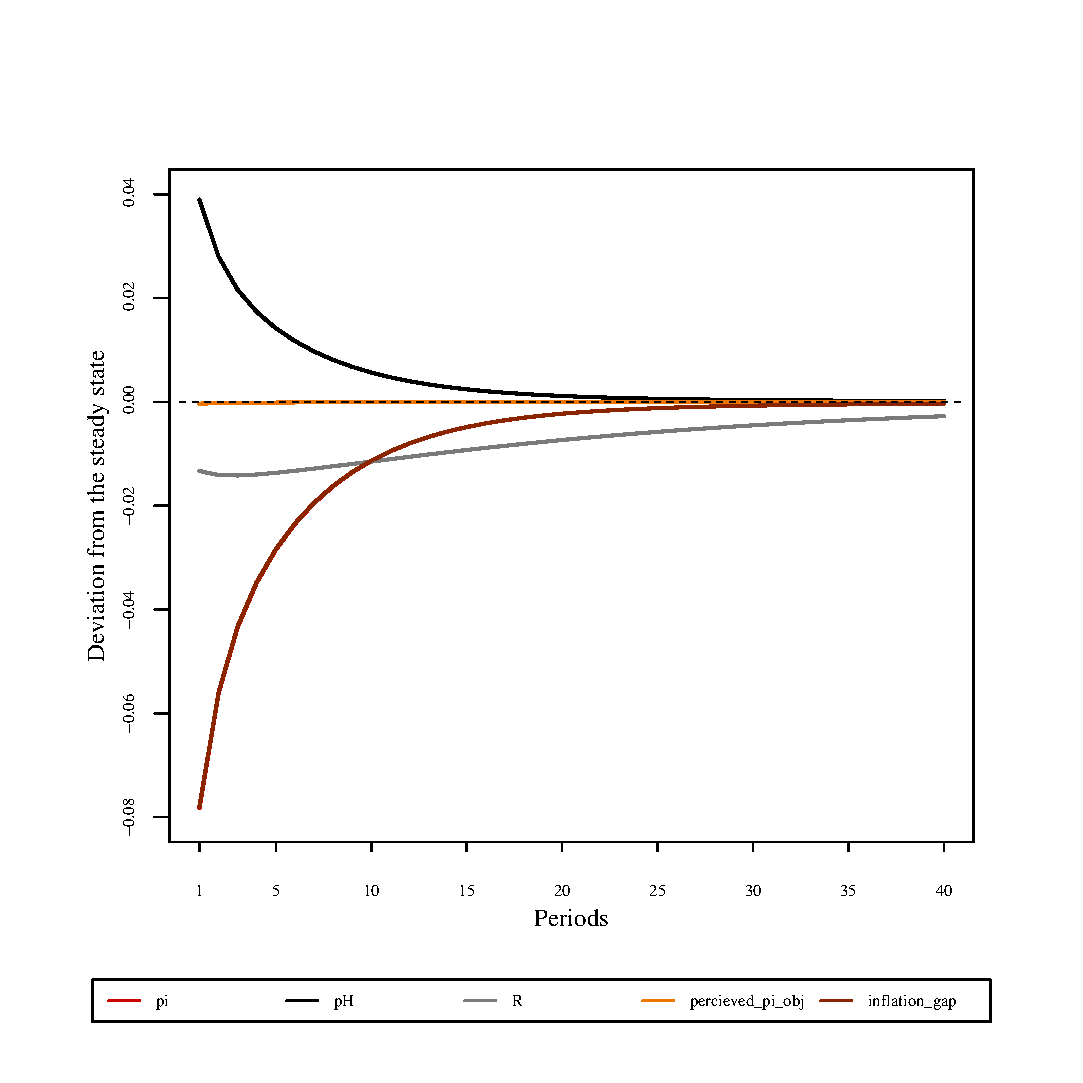
\includegraphics[width=0.99\textwidth, scale=0.55]{plots/plot_131.eps}
\caption{Impulse responses ($\pi, {p\!H}, R, {p\!e\!r\!c\!i\!e\!v\!e\!d}^{\pi^{\mathrm{obj}}}, {i\!n\!f\!l\!a\!t\!i\!o\!n}^{\mathrm{gap}}$) to $\epsilon^{\mathrm{Z}}$ shock}
\end{minipage}
\begin{minipage}{0.5\textwidth}
\vspace*{-3em}
\centering
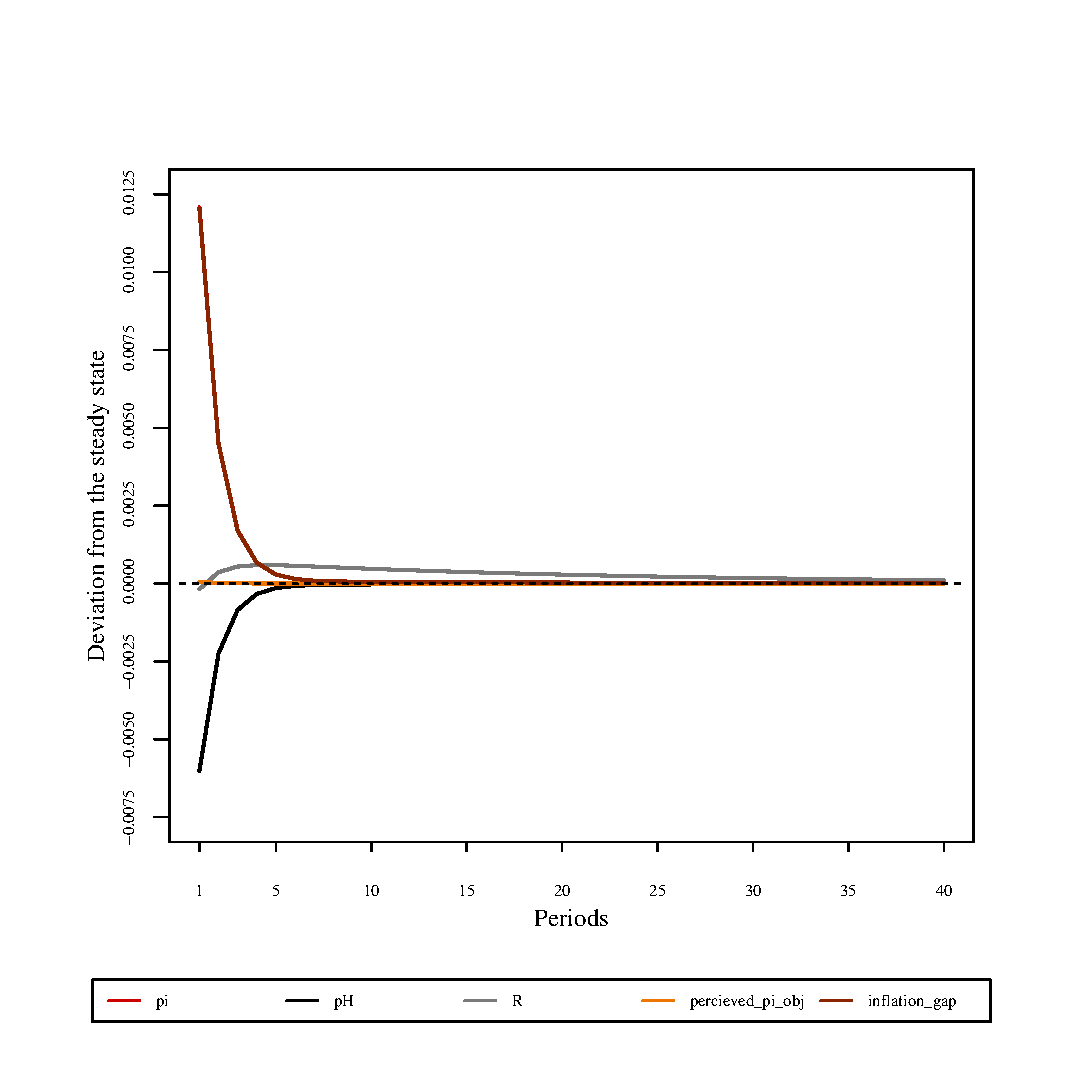
\includegraphics[width=0.99\textwidth, scale=0.55]{plots/plot_132.eps}
\caption{Impulse responses ($\pi, {p\!H}, R, {p\!e\!r\!c\!i\!e\!v\!e\!d}^{\pi^{\mathrm{obj}}}, {i\!n\!f\!l\!a\!t\!i\!o\!n}^{\mathrm{gap}}$) to $\eta^{\mathrm{p}}$ shock}
\end{minipage}
\end{figure}

\begin{figure}[h]
\begin{minipage}{0.5\textwidth}
\vspace*{-3em}
\centering
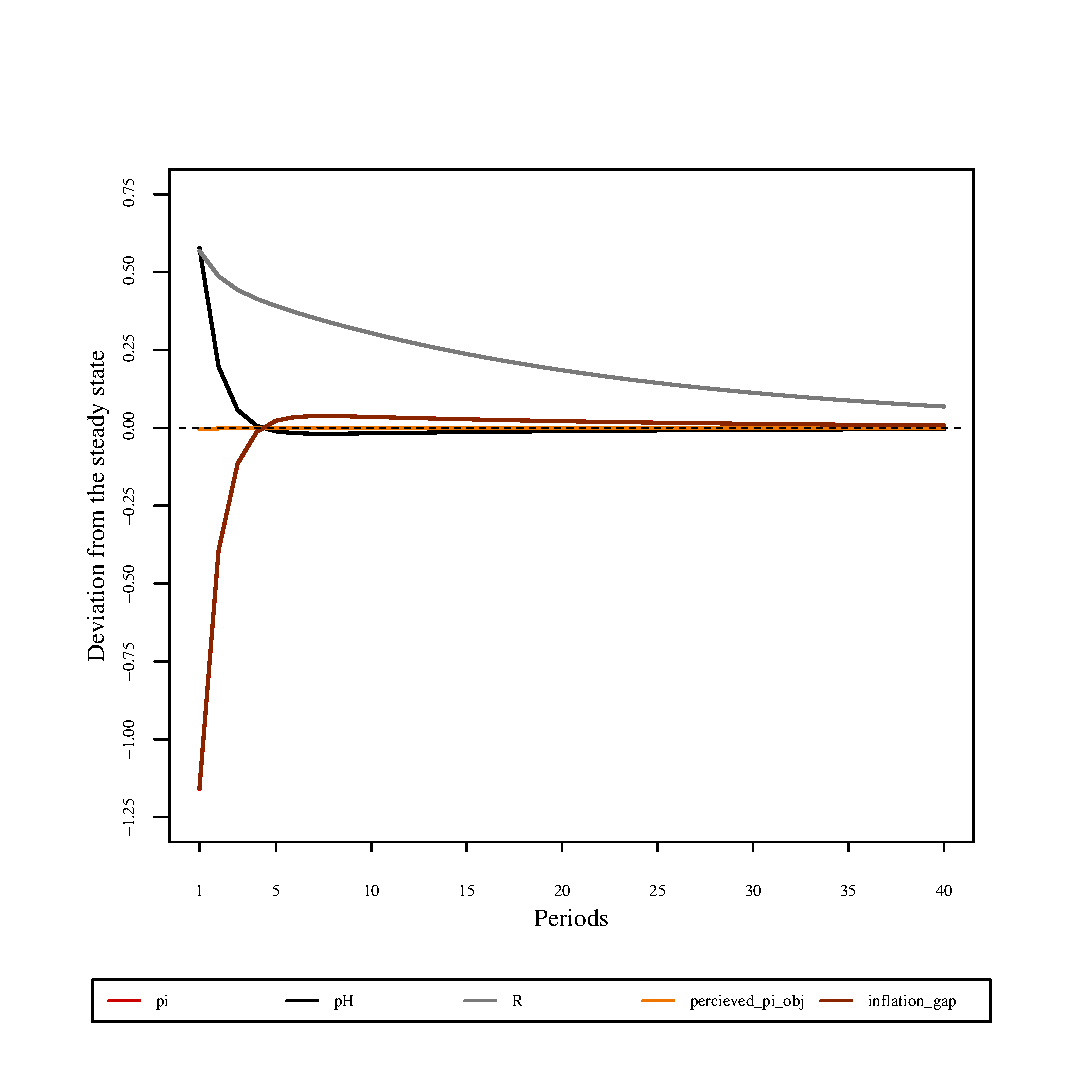
\includegraphics[width=0.99\textwidth, scale=0.55]{plots/plot_133.eps}
\caption{Impulse responses ($\pi, {p\!H}, R, {p\!e\!r\!c\!i\!e\!v\!e\!d}^{\pi^{\mathrm{obj}}}, {i\!n\!f\!l\!a\!t\!i\!o\!n}^{\mathrm{gap}}$) to $\eta^{\mathrm{R}}$ shock}
\end{minipage}
\begin{minipage}{0.5\textwidth}
\vspace*{-3em}
\centering
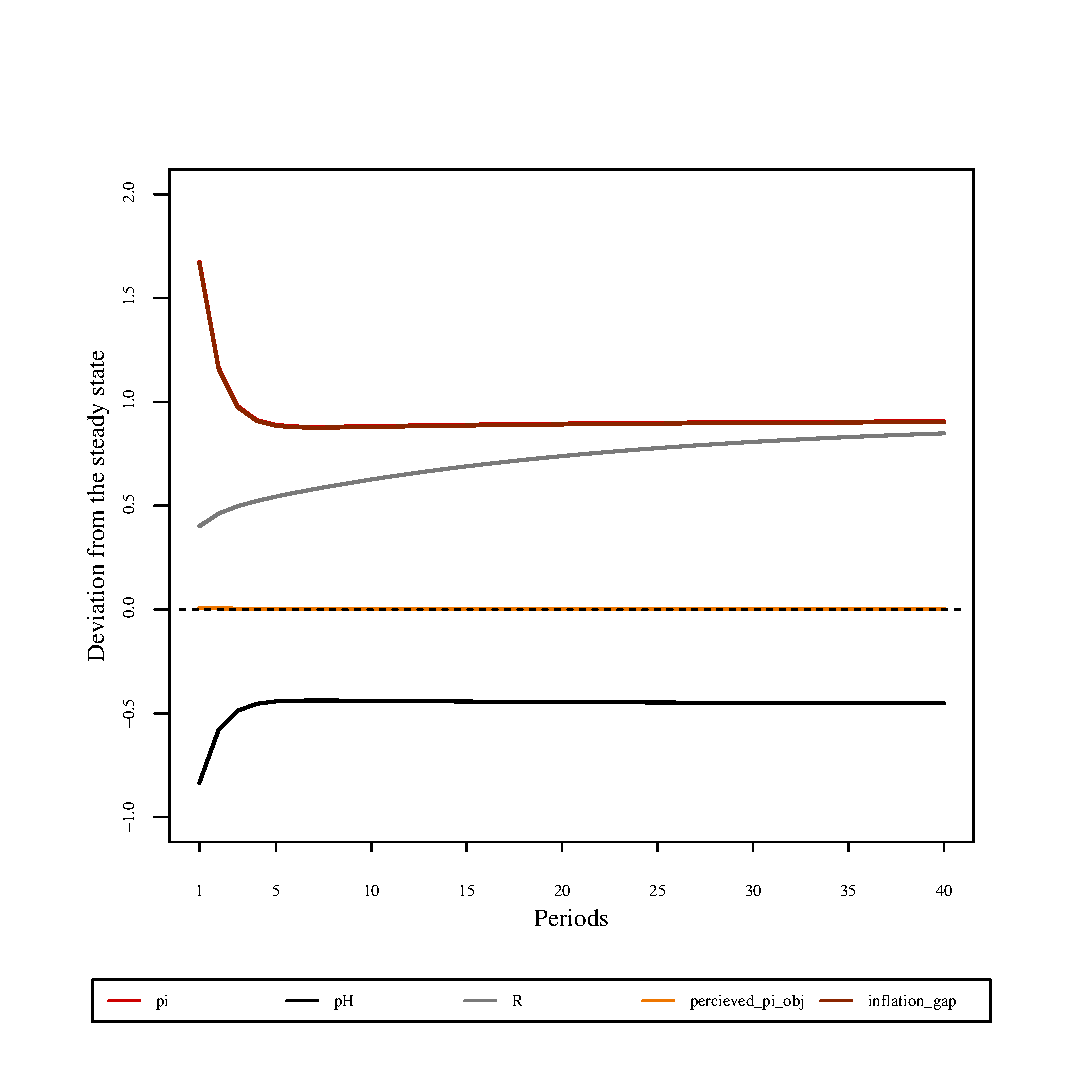
\includegraphics[width=0.99\textwidth, scale=0.55]{plots/plot_134.eps}
\caption{Impulse responses ($\pi, {p\!H}, R, {p\!e\!r\!c\!i\!e\!v\!e\!d}^{\pi^{\mathrm{obj}}}, {i\!n\!f\!l\!a\!t\!i\!o\!n}^{\mathrm{gap}}$) to $\eta^{\pi}$ shock}
\end{minipage}
\end{figure}

\pagebreak

\begin{figure}[h]
\centering
\begin{minipage}{0.5\textwidth}
\vspace*{-3em}
\centering
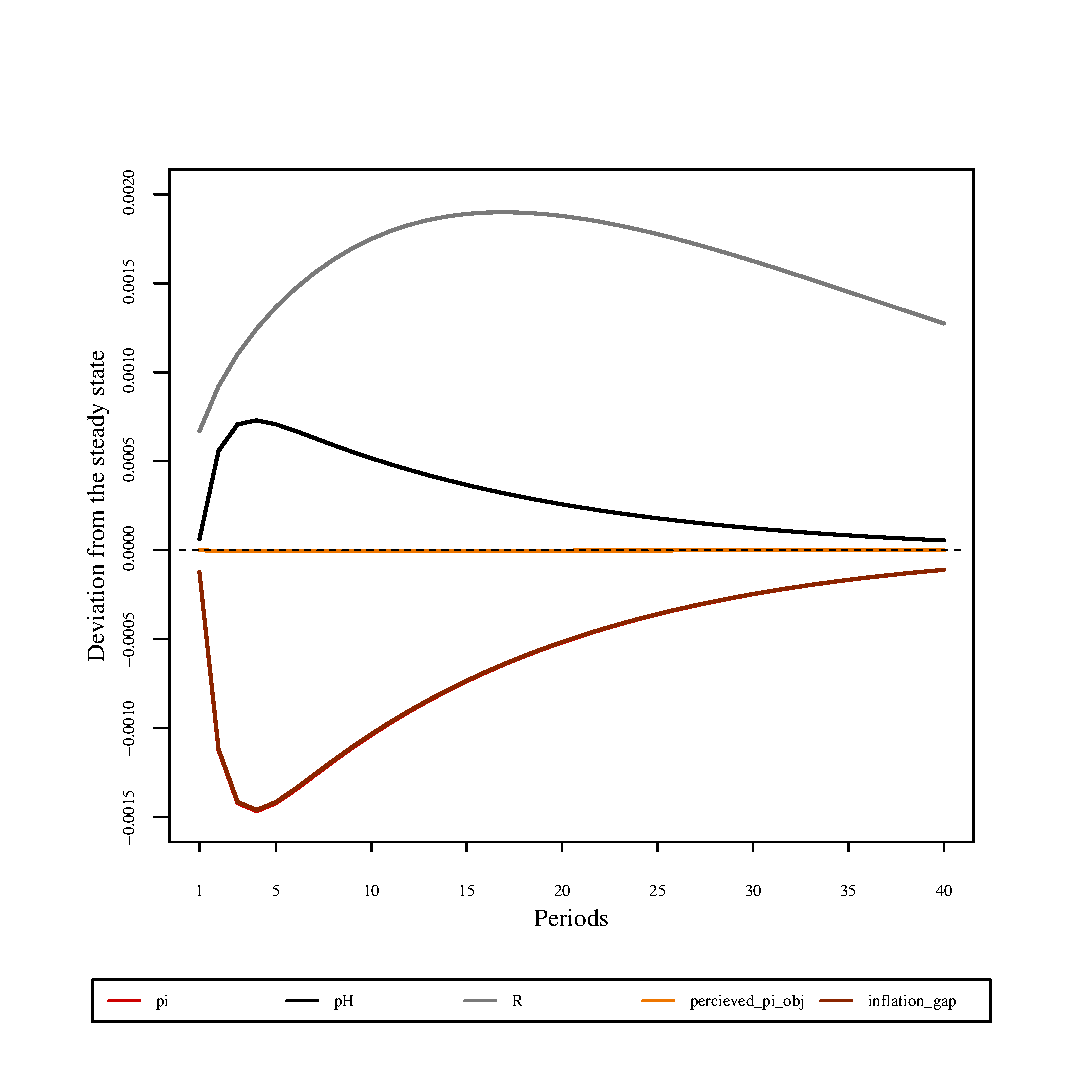
\includegraphics[width=0.99\textwidth, scale=0.55]{plots/plot_135.eps}
\caption{Impulse responses ($\pi, {p\!H}, R, {p\!e\!r\!c\!i\!e\!v\!e\!d}^{\pi^{\mathrm{obj}}}, {i\!n\!f\!l\!a\!t\!i\!o\!n}^{\mathrm{gap}}$) to $\eta^{\mathrm{G}}$ shock}
\end{minipage}
\end{figure}
